\documentclass[12pt, letterpaper]{article}
\usepackage[margin=1in]{geometry}
\usepackage{graphicx}
\usepackage{float}
\usepackage[T1]{fontenc}
\usepackage[polish]{babel}
\usepackage[utf8]{inputenc}
\usepackage{amsmath}
\usepackage{listings, newtxtt}


\graphicspath{{images/}}
\lstset{basicstyle=\ttfamily, keywordstyle=\bfseries}

\title{Teoria współbieżności - lab 5}
\author{Błażej Nowicki}
\date{\today}
\begin{document}
\maketitle
\subsection*{Wstęp}
W języku Python zaimplementowano program, który
dla podanych w pliku konfiguracyjnym produkcji, alfabetu i słowa:
\begin{enumerate}
	\item Wyznacza relację zależności D
	\item Wyznacza relację niezależności I
	\item Wyznacza postać normalną Foaty
	\item Rysuje graph zależności w postaci minimalnej słowa
\end{enumerate}
Dokładny opis implementacji jest dostępny w komentarzach w kodzie źródłowym.
Główną część skryptu zaprezentowano poniżej. Uruchomienie tej części progamu nie wymaga 
instalowania żadnych dependencji. Aby uruchomić opcjonalne rysowanie grafu zależności 
(oprócz domyślnego wypisania formatu dot) należy doinstalować moduł graphviz. \\
`pip install graphviz`
\begin{lstlisting}[language=Python]
    from utils import *
    import os

    # Read configuration file
    directory = "sample_inputs"
    file_name = "sample1.txt"
    with open(os.path.join(directory, file_name)) as f:
        input = f.read()

    # Extract alphabet and productions from the text 
    parser = Parser(input)
    alphabet = parser.get_alphabet()
    productions = parser.get_productions()
    for production in productions:
        print(production)

    # Define both dependency and independency relations
    relation = Relation(productions, alphabet)
    print(relation.get_dependencies_str())
    print(relation.get_independencies_str())

    # Create graph for given word and calculate Foata Normal Form
    word = parser.get_word()
    graph = Graph(relation, word)
    print(graph.FNF())
    print(graph)
\end{lstlisting}
\subsection*{Przykład 1}
Plik wejściowy
\begin{lstlisting}
    (a) x := x + y
    (b) y := y + 2z
    (c) x := 3x + z
    (d) z := y - z

    A = {a, b, c, d}

    w = baadbc
\end{lstlisting}
Wynik działania programu
\begin{lstlisting}
    (a) x <- x, y
    (b) y <- y, z
    (c) x <- x, z
    (d) z <- y, z

    D = {(a,a),(a,b),(a,c),(b,a),(b,b),(b,d),(c,a),(c,c),(c,d),(d,b),(d,c),(d,d)}
    I = {(a,d),(b,c),(c,b),(d,a)}

    FNF([w]) = (b)(ad)(a)(bc)

    digraph g{
    1 -> 2
    2 -> 3
    1 -> 4
    3 -> 5
    4 -> 5
    3 -> 6
    4 -> 6
    1[label=b]
    2[label=a]
    3[label=a]
    4[label=d]
    5[label=b]
    6[label=c]
    }
\end{lstlisting}
Wygenerowany graf
\begin{figure}[H]
    \centering
    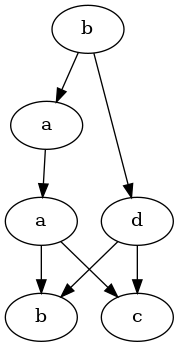
\includegraphics[width=0.2\textwidth]{graph.png}
    \caption{Graf zależności}
\end{figure}
\subsection*{Przykład 2}
Plik wejściowy
\begin{lstlisting}
    (a) x := x + 1
    (b) y := y + 2z
    (c) x := 3x + z
    (d) w := w + v
    (e) z := y - z
    (f) v := x + v

    A = {a, b, c, d, e, f}
    w = acdcfbbe
\end{lstlisting}
Wynik działania programu
\begin{lstlisting}
    (a) x <- x
    (b) y <- y, z
    (c) x <- x, z
    (d) w <- w, v
    (e) z <- y, z
    (f) v <- x, v
    D = {(a,a),(a,c),(a,f),(b,b),(b,e),(c,a),(c,c),(c,e),(c,f),(d,d),(d,f),(e,b),(e,c),(e,e),(f,a),(f,c),(f,d),(f,f)}
    I = {(a,b),(a,d),(a,e),(b,a),(b,c),(b,d),(b,f),(c,b),(c,d),(d,a),(d,b),(d,c),(d,e),(e,a),(e,d),(e,f),(f,b),(f,e)}
    FNF([w]) = (adb)(cb)(c)(fe)
    digraph g{
    1 -> 2
    2 -> 4
    3 -> 5
    4 -> 5
    6 -> 7
    4 -> 8
    7 -> 8
    1[label=a]
    2[label=c]
    3[label=d]
    4[label=c]
    5[label=f]
    6[label=b]
    7[label=b]
    8[label=e]
    }
\end{lstlisting}
Wygenerowany graf
\begin{figure}[H]
    \centering
    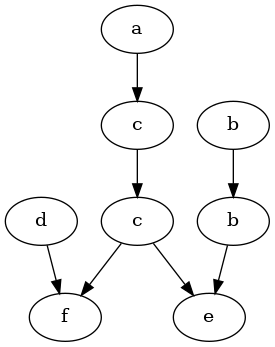
\includegraphics[width=0.4\textwidth]{graph2.png}
    \caption{Graf zależności}
\end{figure}
\end{document}